\section{Methodology}

\subsection{Backbone Model: ResNet-18}

% explain what is ResNet-18

ResNet-18 is a convolutional neural network (CNN) that is used as a backbone model in this project. The architecture can be illustrated as figure \ref{fig:resnet18} \cite{ResNet-18}.
It is a 18-layer deep neural network that is trained on the ImageNet dataset. The ImageNet dataset is a large dataset that contains 1.2 million images with 1000 classes. The ResNet-18 model is trained on the ImageNet dataset to classify the images into 1000 classes.

% insert the ResNet-18 picture

\begin{figure}[h]
\centering
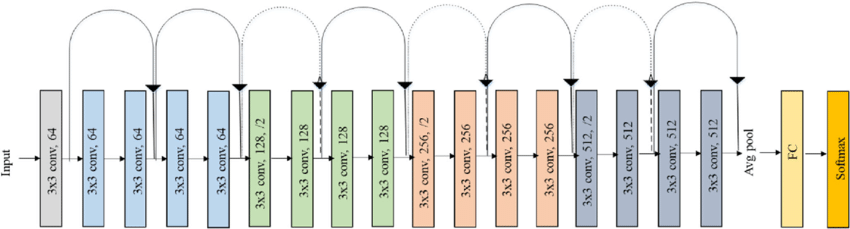
\includegraphics[width=1\textwidth]{ResNet18.png}
\caption{ResNet-18 Architecture}
\label{fig:resnet18}
\end{figure}

\subsection{Adversarial Attacks}

% explain what is adversarial attacking

Adversarial attacking is a technique that can be used to fool machine learning models. It is a type of attack that aims to change the input data in a way that the model will misclassify it. The adversarial attacking technique is based on the fact that machine learning models are vulnerable to small perturbations in the input data. The perturbations are usually imperceptible to the human eye, but they can cause the model to misclassify the input data.

Adversarial examples are hard to defend against because it is difficult to construct a theoretical model of the adversarial example crafting process. Adversarial examples are solutions to an optimization problem that is non-linear and non-convex for many ML models, including neural networks. Because we don't have good theoretical tools for describing the solutions to these complicated optimization problems, it is very hard to make any kind of theoretical argument that a defense will rule out a set of adversarial examples.

\begin{figure}[h]
    \centering
    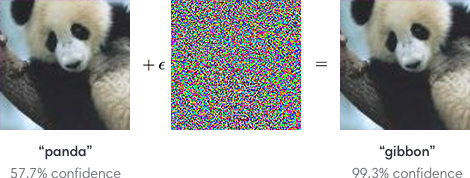
\includegraphics[width=0.8\textwidth]{adversarial_attack.png}
    \caption{An adversarial input, overlaid on a typical image, can cause a classifier to miscategorize a panda as a gibbon.}
    \label{fig:adversarial_attack}
\end{figure}
    

Another reason is they require machine learning models to produce good outputs for every possible input. Most of the time, machine learning models work very well but only work on a very small amount of all the many possible inputs they might encounter. \cite{adversarial_2020}

\subsection{PGD Attack}

The PGD attack is a white-box attack which means the attacker has access to the model gradients i.e. it knows every weight in ResNet-18 in our project. This model gives the attacker much more power than black box attacks as they can specifically craft their attack to fool the face recognition model without having to rely on transfer attacks that often result in human-visible perturbations. PGD can be considered the most “complete” white-box adversary as it lifts any constraints on the amount of time and effort the attacker can put into finding the best attack. \cite{knagg_2019}